\documentclass[10pt,a4paper,final]{article}
\usepackage[utf8]{inputenc}
\usepackage[francais]{babel}
\usepackage[T1]{fontenc}
\usepackage{amsmath}
\usepackage{amsfonts}
\usepackage{graphicx}
\usepackage{amssymb}
\usepackage{lmodern}
\usepackage[table,xcdraw]{xcolor}
\author{Òsca-Font dubèrta}
\thispagestyle{empty}

\begin{document}


\begin{center}

\includegraphics[height=50pt]{PWD/verboc_oc.eps}
\end{center}

\begin{center}
\huge{Conjugador Dialect}
\end{center}

\section*{Vèrb}
\subsection*{Modèl}
\subsection*{DefMdl}
\begin{tabular}{|c|c|c|c|c|}
\hline 
\multicolumn{5}{|c|}{\textbf{Indicatiu}} \\ 
\hline 
 & \textbf{Present} & \textbf{Imperfach} & \textbf{Preterit} & \textbf{Futur} \\ 
\hline 
\textit{s1} & prsS1 & imfS1 & prtS1 & ftrS1 \\ 
\hline 
\textit{s2} & prsS2 & imfS2 & prtS2 & ftrS2 \\ 
\hline 
\textit{s3} & prsS3 & imfS3 & prtS3 & ftrS3 \\ 
\hline 
\textit{p1} & prsP1 & imfP1 & prtP1 & ftrP1 \\ 
\hline 
\textit{p2} & prsP2 & imfP2 & prtP2 & ftrP2 \\ 
\hline 
\textit{p3} & prsP3 & imfP3 & prtP3 & ftrP3 \\ 
\hline 
\multicolumn{5}{|c|}{} \\ 
\hline 
 & \multicolumn{2}{c|}{\textbf{Subjontiu}}  & \multicolumn{2}{c|}{\textbf{Imperatiu}} \\ 
\hline 
 & \textbf{Present} & \textbf{Imperfach} & \textbf{Forma affirmativa} & \textbf{Forma negativa} \\ 
\hline 
\textit{s1} & supS1 & suiS1 & \multicolumn{2}{c|}{} \\ 
\hline 
\textit{s2} & supS2 & suiS2 & impS2 & imnS2 \\ 
\hline 
\textit{s3} & supS3 & suiS3 & \multicolumn{2}{c|}{} \\ 
\hline 
\textit{p1} & supP1 & suiP1 & impP1 & imnP1 \\ 
\hline 
\textit{p2} & supP2 & suiP2 & impP2 & imnP2 \\ 
\hline 
\textit{p3} & supP3 & suiP3 & \multicolumn{2}{c|}{} \\ 
\hline 
\multicolumn{5}{|c|}{} \\ 
\hline 
 & \multicolumn{2}{c|}{\textbf{Conditional}} & \multicolumn{2}{c|}{} \\ 
\hline 
 &  \multicolumn{2}{c|}{\textbf{Present}} & \multicolumn{2}{c|}{\textbf{Formas impersonalas}}  \\ 
\hline 
\textit{s1} & \multicolumn{2}{c|}{cndS1}  & \textbf{Infinitiu} & infFI \\ 
\hline 
\textit{s2} & \multicolumn{2}{c|}{cndS2}  & \textbf{Gerondiu} & gerFI \\ 
\hline 
\textit{s3} & \multicolumn{2}{c|}{cndS3}  & \textbf{Participi passat} & pamFI / pafFI \\ 
\hline 
\textit{p1} & \multicolumn{2}{c|}{cndP1} & \multicolumn{2}{c|}{} \\ 
\hline 
\textit{p2} & \multicolumn{2}{c|}{cndP2} & \multicolumn{2}{c|}{} \\ 
\hline 
\textit{p3} & \multicolumn{2}{c|}{cndP3} & \multicolumn{2}{c|}{} \\ 
\hline 
\end{tabular}


\includegraphics[width=40pt]{PWD/QRCode_loCongres.eps}\hfill\includegraphics[width=40pt]{PWD/by-sa.eps}

\begin{center}

\includegraphics[width=100pt]{PWD/logoCongres300.jpg}
\end{center}

\footnotesize{CREDITS}

\end{document}


